% Drawing 141/01-14 -- folder 141, batch 01, archive page 14 (PDF page 15).
% Transcription: à droite, quatre figures de lacets dans le plan. En haut : deux points $i$ et $-i$ l'un au-dessus de l'autre, reliés par deux arcs en croissant, et chacun relié par un trait double à un gros point cerclé à droite ; une longue ligne fine horizontale traverse la figure. Au milieu à gauche : $i$ en haut, $-i$ en bas, $0$ entouré d'une boucle sur un axe horizontal gradué en $1$, un trait descendant de $i$ à la boucle, un trait double de la boucle à $-i$, et deux grands arcs de $i$ à $-i$ passant à droite de $0$. Au milieu à droite : un lacet en « V » à trait double finissant par un petit cercle, avec les lettres $0$ et $1$. En bas à droite : un lacet en équerre à trait double, entourant un point et finissant par un petit cercle.
% Kind: four figures of loops in the plane round 0 and 1, based at i and -i. Method 2 (schematic redraw from the facsimile). Status: partial.
% Notes: Four figures. (1) Top: the points i (top) and its mate below (-i, label not legible), two crescent arcs between them, a double stroke from each to the heavy ringed point at the right (a letter is scribbled inside it: not read), an arrowhead on the upper double stroke near i; the long thin horizontal line across the figure with a dot on it. (2) Middle left: i, -i, the loop round 0 on the horizontal axis, the tick and the label 1 on the axis, the stroke from i down to the loop, the double stroke from the loop down to -i, and the two large arcs from i to -i on the right of 0 (the inner one ends just above -i). (3) Middle right: a V of double strokes, from the top down to its tip and up to a small circle at the right, with the letters 0 (at the left) and 1 (inside the V). (4) Bottom right: an L of double strokes, coming down, turning round a point inside a small loop, and running right to a small circle. Left out: the faint pencil ovals round 0 in (2), two small dots near -i, the scribble inside the ringed point of (1). Still differs: double strokes are drawn as two parallel lines read on the crop, their closures at the ends are approximate; in (3) the letters are small and their reading (0, 1) is not sure. Redrawn 2026-11-12 (issue 128): to check again.
% Coordinates: 1 unit = 1 mm = 1/100 of the crop width (bbox in page fractions: [0.6, 0.06, 0.93, 0.33]).
% Redrawn by Claude (claude-fable-5-2), issue #128, 2026-11-12; not checked by a human; not compiled (no TeX in the session).
% Rights: reproduces part of the work -- behind RENDER_TRANSCRIPTS, never published by itself.
\documentclass[tikz,border=3pt]{standalone}
\usepackage{amsmath,amssymb}
\usetikzlibrary{patterns,arrows.meta}
\tikzset{pencil/.style={black!45}, struck/.style={black!35}, mpt/.style={circle,draw,inner sep=1.3pt}, pt/.style={circle,fill,inner sep=0.9pt}, opt/.style={circle,draw,fill=white,inner sep=1.1pt}}
\begin{document}
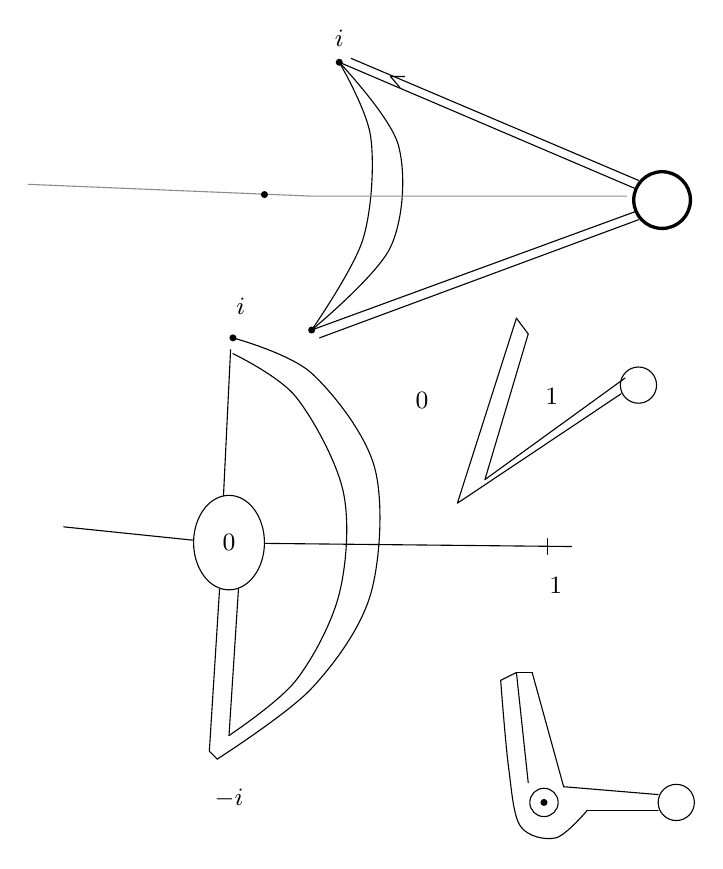
\begin{tikzpicture}[x=1mm,y=1mm,line cap=round,line join=round,font=\scriptsize]
\node[pt] at (43.5,-10.5) {};
\node[pt] at (40,-44.5) {};
\node[inner sep=1pt] at (43.5,-7.5) {\small $i$};
\draw plot[smooth, tension=0.55] coordinates {(43.5,-10.5) (47.5,-20) (46.5,-33) (40,-44.5)};
\draw plot[smooth, tension=0.55] coordinates {(43.5,-10.5) (51,-21) (50,-34) (40,-44.5)};
\draw (43.5,-10.5) -- (81,-26.5);
\draw (45,-10) -- (81.5,-25.5);
\draw (51.2,-13.7) -- (50,-12.3) -- (51.8,-12.3);
\draw (40,-44.5) -- (81,-29.5);
\draw (41,-45.5) -- (81.5,-30.5);
\draw[very thick] (84.5,-28) circle[radius=3.6];
\draw[pencil] (4,-26) -- (40,-27.5) -- (80,-27.5);
\node[pt] at (34,-27.3) {};
\node[pt] at (30,-45.5) {};
\node[inner sep=1pt] at (31,-41.5) {\small $i$};
\node[inner sep=1pt] at (29.5,-104) {\small $-i$};
\draw (29.5,-71.5) ellipse[x radius=4.5, y radius=6];
\node[inner sep=1pt] at (29.5,-71.5) {\small $0$};
\draw (8.5,-69.5) -- (25,-71.2);
\draw (34,-71.6) -- (73,-72);
\draw (70,-71) -- (70,-73);
\node[inner sep=1pt] at (71,-77) {\small $1$};
\draw (29.7,-47) -- (28.8,-65.5);
\draw (28.3,-77.4) -- (27,-98);
\draw (30.7,-77.4) -- (29.5,-96);
\draw (27,-98) -- (28,-99);
\draw plot[smooth, tension=0.55] coordinates {(30,-45.5) (40,-50) (48,-62) (47.5,-78) (40,-90) (28,-99)};
\draw plot[smooth, tension=0.55] coordinates {(30,-47.5) (38,-53) (44,-65) (43.5,-78) (38,-89) (29.5,-96)};
\draw (66,-43) -- (58.5,-66.5) -- (79.3,-52.6);
\draw (67.5,-45) -- (62,-63.5) -- (79.8,-50.6);
\draw (66,-43) -- (67.5,-45);
\draw (81.5,-51.5) circle[radius=2.3];
\node[inner sep=1pt] at (54,-53.5) {\small $0$};
\node[inner sep=1pt] at (70.5,-53) {\small $1$};
\draw plot[smooth, tension=0.55] coordinates {(64,-89) (65,-100) (66.5,-107.5) (71,-109) (75,-105.5)};
\draw (75,-105.5) -- (84,-105.5);
\draw (66,-88) -- (68,-88);
\draw (66,-88) -- (67.5,-102);
\draw (68,-88) -- (72,-102.5) -- (84,-103.5);
\draw (64,-89) -- (66,-88);
\draw (69.5,-104.5) circle[radius=1.8];
\node[pt] at (69.5,-104.5) {};
\draw (86.3,-104.5) circle[radius=2.3];
\end{tikzpicture}
\end{document}
